\chapter{Experiment 2: validation of remote detection of emotions}
\label{ch:experiment2}

The first conducted experiment aimed at gathering data and exploring the relations regarding facial actions (FA), HR and emotional states, particularly stress and boredom. The experiment is based on the previously mentioned findings that HR varies according to stress/frustration and that facial expressions can convey contextual information about emotional state \parencite{giannakakis2017stress}. As opposed to previously mentioned works, in this experiment each subject spends an average of 25 minutes in the session, playing three different games that were custom-made to provoke the emotional reactions similar to off-the-shelf games. Subjects were also not instructed regarding how they should move, so body and facial reactions are likely to be the ones the subject would normally perform under a gaming context. The approach consists of using induced boring to stressful mechanics in the games to produce variations in the emotional state and HR of participants. %, based on the previously mentioned findings that HR varies according to stress/frustrations.

%FA were manually detected and annotated based on observations.
In total, three studies were performed on the data obtained from the experiment. The first study focuses on empirical exploration of how FA, defined as being any facial movement different from a neutral face, e.g. lips contraction, relate to emotional states. The second study focuses on the variations of HR that occurred during the interaction with the games, specially under situations that were designed to provoke boredom and stress. It should confirm the hypothesis that the HR during boring and stressful parts of a game is in fact different. Finally the third study focuses on the accuracy evaluation of an rPPG technique when applied to gaming sessions where subjects behave naturally.

The following sections present information regarding the participants, the experiment structure and each one of the mentioned studies.

%%%%%%%%%%%%%%%%%%%%%%%%%%%%%%%%%%%%%%%%%%%%%%%%%%%%%%%%%%%%%%%%%%%%%%%%%%%%%%%%%%%%%%%
\section{Method}
%%%%%%%%%%%%%%%%%%%%%%%%%%%%%%%%%%%%%%%%%%%%%%%%%%%%%%%%%%%%%%%%%%%%%%%%%%%%%%%%%%%%%%%

%%%%%%%%%%%%%%%%%%%%%%%%%%%%%%%%%%%%%%%%%%%%%%%%%%%%%%%%%%%%%%%%%%%%%%%%%%%%%%%%%%%%%%%
\subsection{Experimental procedure}

Twenty adult participants of both genders (10 female) with different ages (22 to 59, mean 35.4, SD 10.79) and different gaming experience gave their informed and written consent to participate in the experiment. The study population consisted of staff members and students of the University of Sk\"ovde, as well as citizens of the community/city. When asked how skilled subjects believe they are at playing video games, 1 subject (5\%) reported no skill, 10 (50\%) reported not very skilled, 7 (35\%) reported moderately skilled and 2 (10\%) reported very skilled. When asked the number of hours per week they had played any type of video game over the last year, 2 subjects (10\%) reported more than 10, 6 (30\%) reported 5 to 10, 2 (10\%) reported 3 to 4, 2 (10\%) reported 1 to 3, 4 (20\%) reported 0 to 1, and 4 (20\%) reported no activity. Those numbers indicate that the population has a diversity of gaming experience and playing frequency, which provides the experiment with information that is less skewed towards specific profile of players, e.g. hardcore players.

Subjects were seated in front a computer, alone in the room, while being recorded by a camera and measured by a heart rate sensor. The camera was attached to a tripod placed in front of the subjects at approximately 0.6m of distance; the camera was slightly tilted up. A spotlight, tilted 45$^{\circ}$ up, placed at a distance of 1.6m from the subject and 45cm higher than the camera level, was used for illumination; no other light source was active during the experiment. Figure \ref{fig:setup} illustrates the setup.

\begin{figure}[h]
\centering
\includegraphics[width=\textwidth]{figures/experiment-setup-double}
\caption{Experiment setup. On the left, illustration regarding the position of equipment, including the angle of the external light source. On the right, highlight of the position and angle of the video camera.}
\label{fig:setup}
\end{figure}

The participants were each recorded for about 25 minutes, during which they played three games. Each game was followed by a questionnaire related to the game and stress/boredom. The first two games were followed by a 138 seconds rest period, where the subjects listened to calm classic music. The last game was followed by an additional questionnaire about age and gaming experience/profile. The order which the games were played was randomized among subjects. Participants received instructions from a researcher that they should play three games, answer a questionnaire after each game and rest; they were told that their gaming performance was not being analyzed, that they should not give up in the middle of the games and that they should remain seated during the whole process.

\subsubsection{Calibration games}

The three games\footnote{Source code available at: https://github.com/Dovyski/face-tracking-games} used in the experiment were 2D and casual-themed, played with mouse or keyboard in a web browser. The games were carefully designed to provoke boredom at the beginning and stress at the end, with a linear progression between the two states (adjustments of such progression are performed every 1 minute). The game mechanics were chosen based on the capacity to fulfill such linear progression, along with the quality of not allowing the player to instantly kill the main character (by mistake or not), e.g. by falling into a hole. The mechanics were also designed/selected to ensure that all subjects would have the same game pace, e.g. a player must not be able to deliberately control the game speed based on his/her will or skill level.

The \textbf{Mushroom} game, illustrated in Figure \ref{fig:mushroom-platformer-tetris} (left), is a puzzle where the player must feed a character by dragging and dropping mushrooms in rounds. In a given round, $M$ mushrooms are displayed in a grid and the player has $K$ seconds (a decreasing time bar at the top informs the remaining time) to collect good and discard bad (poisonous) mushrooms. At the upper-right corner of the screen, a sign informs the player about the bad/poisonous mushroom of the round. The player must drag and drop all good mushrooms (the ones different from the poisonous indication) into the character, while dragging and dropping the bad ones into the trash can. Mushrooms are differentiated by the colors of their features (circles). The player is rewarded with score points, a health bar increase ($HB\textsubscript{I}$) and a pleasant sound when a right move is performed. In case of mistake a health bar decrease ($HB\textsubscript{D}$) and an annoying/aggressive alarm sound is applied. If the time $K$ is over and the player has not finished moving all the mushroom of the round, each remaining mushroom in the grid is counted as a mistake. If the grid is clean and there is still time available, the player must wait until the time is over. The values of $M$, $K$, $HB\textsubscript{I}$ and $HB\textsubscript{D}$ are used to induce boredom/stress. At the beginning, $M$ is low (starts with 2) and $K$ is high (starts with 45 seconds), so the player spends a significant amount of time waiting for the game to continue; every 1 minute the value of $M$ is increased and $K$ is decreased. The changes continue to happen until the player is unable to deal with the amount of mushrooms within the available time. This leads to mistakes that will eventually decrease the health bar to zero, terminating the game. After the mark of 6 minutes, the game becomes virtually impossible to beat.

The \textbf{Platformer}, illustrated in Figure \ref{fig:mushroom-platformer-tetris} (center), is a side-scrolling, endless runner game where the player must control the main character while collecting hearts and avoiding obstacles (skulls with spikes). The character can jump (by pressing the up arrow key in the keyboard) or slash (S key), however the player is not able to move the main character left or right, it remains in the same position on the screen (towards the left side of the screen). The character moves on top of platforms, which are always perfectly connected, so there are no gaps (holes) among them; the height of the platform can vary, however, so there might be a slope up/down connecting two platforms, for instance. If the character hits an obstacle, the health bar is decreased ($HB\textsubscript{D}$) and a sound effect related to pain is played. If any heart is collected, the health bar increases ($HB\textsubscript{I}$) and a pleasant sound effect is played. The position where the hearts appear on each platform is adjustable (defined by $HH$), so they can appear close to the platform (no action is required to collect the heart) or a bit higher from the ground (jump action is required to collect the heart). The speed of the character ($S$, which is the velocity at which elements are moving on the screen), the height variation of each new platform that appears on the screen ($HV$), the amount of hearts ($G$) and obstacles ($E$) per platform are all controlled by the game and used to adjust boredom/stress. At the beginning, boredom is induced by keeping all previously mentioned parameters with low values, which means the game is slow, the character moves from platform to platform at the same height and almost no hearts or obstacles appear on the screen. The few hearts that are available are placed close to the ground to destimulate jumping actions. As time progresses, the values of $S$, $E$, $HV$, $HB\textsubscript{D}$ and $HH$ increase, while $G$ and $HB\textsubscript{I}$ decrease to induce the player to a stressfull state. At the mark of 5 minutes, for instance, the game is significantly fast, with several obstacles on the screen and almost no hearts to collect; the damage caused to the character when hit by an obstacle is also higher than the beginning of the game. The linear increase in difficulty will eventually result in consecutive hits (mistakes), which will decrease the health points until zero, when the game ends.

\begin{figure*}[!h]
\centering
\includegraphics[width=\textwidth]{figures/experiment1-games}
\caption{Mushroom (left), Platformer (center) and Tetris (right). In Mushroom, player has to drag and drop the correct mushrooms into the character, discarding the wrong ones into the trash. In Platformer, the player has to jump over or slide under obstacles while collecting hearts. In our version of Tetris, there are no hints about the next piece to be added to the screen}
\label{fig:mushroom-platformer-tetris}
\end{figure*}

Finally the game \textbf{Tetris}, shown in Figure \ref{fig:mushroom-platformer-tetris} (right), is a modification of the original Tetris game. In our version of the game, the next block to be added to the screen is not displayed, so the player is unable to predict future moves. Additionally, the down key, usually used to speed up the descendant trajectory of the current piece, is disabled. The keyboard controls are the arrow keys to move the piece left/right and the R key to rotate the piece. The game is also modified to ensure that all subjects received the same sequence of pieces (we use the same seed for the generation of random numbers). The speed that the pieces fall ($S$) is used to control boredom and stress; at the beginning of the game, boredom is induced by using a low value for $S$, which makes the game slow since the pieces are falling slowly and the player is unable to speed them up. As time progresses, $S$ increases linearly making the game faster and harder to play, which should induce stress. At the mark of 5 minutes, for instance, a single piece takes almost 1 second to traverse the whole screen.

\subsubsection{Evaluation game}
Explain the Mario game.

\subsubsection{Data collection}

During the whole experiment, subjects were recorded using a Canon Legria HF R606 video camera. All videos were recorded in color (24-bit RGB with three channels $\times$ 8bits/channel) at 50p frames per second (fps) with pixel resolution of 1920 $\times$ 1080 and saved in AVCHD-HD format, MPEG-4 AVC as the codec. At the same time, subject's HR was measured by a TomTom Runner Cardio watch (TomTom International BV, Amsterdam, Netherlands), which was used as ground truth. The watch was placed on the left arm, approximately 7cm away from the wrist, like a regular wrist watch, and its use was unobtrusive, so it did not affect the movements of the subjects, who could still use both hands to play the games. The watch recorded the HR at 1 Hz.

After each game, subjects answered a questionnaire in order to provide self-reported stress and bordeom measurements. The questionnaire had six questions: the first four were a 5-point Likert scale related to how the player felt related to stress/boredom at the beginning/end of each game (1: not stressed/bored at all, 5: extremely stressed/bored); a question to identify the part of the game that best describes the moment the subject enjoyed the most (very beginning, after beginning and before middle, middle, after middle and before end, very end); finally a question asking if the subject understood the game. Before the end of the experiment, subjects answered a final questionnaire with nine questions, which were related to: age; gender; number of hours per week spent with games over the last year (question from the video game experience questionnaire \parencite{unsworth2015playing}); how proficient or skilled the subject believe being at playing video games (question from the Survey of Spatial Representation and Activities - SSRA \parencite{terlecki2005important}); familiarity with puzzle, platform and Tetris games; current state of mind compared to other days (e.g. normal, unusually stressed, etc.); and gaming profile (like, dislike challenging games).


%%%%%%%%%%%%%%%%%%%%%%%%%%%%%%%%%%%%%%%%%%%%%%%%%%%%%%%%%%%%%%%%%%%%%%%%%%%%%%%%%%%%%%%
\subsection{Emotion estimation}

\subsubsection{Data preprocessing}
Explain how the data from the calibration games were split into 3 pieces and the middle one was discarded. Also explain that Mario levels whose stress/boredom levels were equal were discarded.

\subsubsection{Relevant feature extraction}
Explain about how the features used to train the machine learning model were extracted, e.g. facial features, remote HR.

\subsubsection{Emotion classification}
Explain how the machine learning model, i.e. neural network, was trained and designed.

\subsubsection{Evaluation of emotion classification}
Explain how the machine learning model was applied to the COTS levels to estimate their emotional state.

%%%%%%%%%%%%%%%%%%%%%%%%%%%%%%%%%%%%%%%%%%%%%%%%%%%%%%%%%%%%%%%%%%%%%%%%%%%%%%%%%%%%%%%
\subsection{Analysis}
%%%%%%%%%%%%%%%%%%%%%%%%%%%%%%%%%%%%%%%%%%%%%%%%%%%%%%%%%%%%%%%%%%%%%%%%%%%%%%%%%%%%%%%

Additionally, the validation sampling is every 5 seconds based on \parencite{ravaja20051} (IBI with a peak decrease 4 sec after event onset) and \parencite{valenza2014revealing} (estimating emotions each 10 seconds achieve an overall accuracy in recognizing four emotional states based on the circumplex model of affect of 79.29\%, with 79.15\% on the valence axis, and 83.55\% on the arousal axis).

%%%%%%%%%%%%%%%%%%%%%%%%%%%%%%%%%%%%%%%%%%%%%%%%%%%%%%%%%%%%%%%%%%%%%%%%%%%%%%%%%%%%%%%
\section{Results}
%%%%%%%%%%%%%%%%%%%%%%%%%%%%%%%%%%%%%%%%%%%%%%%%%%%%%%%%%%%%%%%%%%%%%%%%%%%%%%%%%%%%%%%

%%%%%%%%%%%%%%%%%%%%%%%%%%%%%%%%%%%%%%%%%%%%%%%%%%%%%%%%%%%%%%%%%%%%%%%%%%%%%%%%%%%%%%%
\subsection{Self-reported emotional state}
Show some analysis and statistics regarding the games. I can mention the average stress level reported for some Mario legels, which confirms that our design of the game meets our expectations (some levels must be boring and others must be stressful).

%%%%%%%%%%%%%%%%%%%%%%%%%%%%%%%%%%%%%%%%%%%%%%%%%%%%%%%%%%%%%%%%%%%%%%%%%%%%%%%%%%%%%%%
\subsection{Emotion classification}
Show the results of applying the machine learning model to classify the emotional state of subjects.

%%%%%%%%%%%%%%%%%%%%%%%%%%%%%%%%%%%%%%%%%%%%%%%%%%%%%%%%%%%%%%%%%%%%%%%%%%%%%%%%%%%%%%%
\section{Discussion}
Discussion will be focused on the following: 1) was the machine learning model able to detect emotions with accuracy better than chance? 2) was the use of a multimodal approach (foundation of my thesis) better than the use of only facial features (or only HR)?. This section will almost be a replication of the "Study 5", however using the data from the second experiment instead of the first.

%%%%%%%%%%%%%%%%%%%%%%%%%%%%%%%%%%%%%%%%%%%%%%%%%%%%%%%%%%%%%%%%%%%%%%%%%%%%%%%%%%%%%%%
\section{Conclusion}

%The experiment design will be based on a within-subject approach \cite{lane2015online}. In such approach, all participants perform at all levels of the treatment and there are no control groups. It is the opposite of a between-subjects approach, where subjects are divided in more than one group that receive different treatments. In that approach there are special groups, called control groups, that receive no treatment. The comparison between the control groups and the treatment groups ensures internal validity. In the context of this research, physiological signals will be measured, so the division of subjects into more than one group poses a comparison problem. Each individual will inevitably differ from one another regarding physiological signals, such as variations in average HR during rest, for instance. When measuring HR, for instance, some subjects will have higher/lower HR mean than others, independent of the group they are in or the treatment they undergo. To counter that problem, the experiment will use a one-group posttest design \cite{kirk1982experimental}, as illustrated by Figure \ref{fig:experiment}. Using the first row as an example, subject $S_0$ played game $G_a$ as the first level of the treatment, followed by a post-test of that game ($PT_a$), then a rest period. In the second level of the treatment, the subject played game $G_b$, followed by a post-test of that game ($PT_b$), then another rest period. Finally in the third level of the treatment, the subject played game $G_c$ followed by a post-test of that game ($PT_c$).

%\begin{figure}[ht]
%    \centering
%    \includegraphics[scale=0.5]{imgs/experiment-design.png}
%    \caption{One-group posttest experiment design used in this research. $S_j$ represents the $j^{\text{th}}$ subject, $G_i$ represents a game of type $i$, $PT_i$ is the post-test for game $G_i$ and $rest$ is a resting period.}
%    \label{fig:experiment}
%\end{figure}

%By using a one-group posttest design, each individual will perform on all levels of the treatment (play a set of different games). The within-subjects approach ensures that the differences between subjects are not interfering in the comparison, since a subject is being compared to his/herself in the different levels of the treatment. Subjects are not being compared among each other. In essence, each subject is serving as his/her own control group. According to Kirk \cite{kirk1982experimental}, the one-group posttest design should only be used when the researcher knows the mean value of the independent variable when no treatment is in effect. Such information will be obtained during the resting periods of the experiment, where the baseline value for all measured signals can be established for each subject.

%The process of sampling a group of participants for each experiment will follow the convenience sampling approach, a non-probability sampling technique where participants are recruited because of their convenient accessibility/proximity to the researcher. Volunteers will be randomly recruited for each experiment. A probability sampling approach, where each individual of the population has an equal chance of being selected, would be ideal and would strength the external validity of the research. However the costs, logistics and time constraints associated with it makes such approach impractical in the context of this research.







%\section{Experimental validation of the proposed method}
%\label{closing:emotion-detection-experiment}

%After the previous tasks have been completed, the limitations of the remote readings will be known (and mitigated), the set of user signals to be used in the user-tailored model will be defined and a machine learning model to map user signals into emotional states will be selected. In summary the proposed emotion detection process will be structuraly complete, but not validated.

%An experiment involving emotion detection and a commercial off-the-shelf (COTS) game will then be planned and executed to validate the proposed approach. The experiment, referred to as experiment 2 from now on, aims to test the following hypotesis (\textbf{H}):

%\textbf{H: the method proposed by this research (game-calibrated and user-tailored remote detection of emotions) is more accurate at detecting stress/boredom levels of users during the interaction with a COTS game than it is a detection approach solely based on HR measurements that are above/below the user's baseline.}

%The detection method solely based on HR, however, can use different approaches to perform the HR measurements. It can use a physical sensors, e.g. watch, or a remote approach, e.g. rPPG. In that sense, the previously mentioned hypotesis \textbf{H} can be reformulated into two hypotheses, \textbf{H1} and \textbf{H2}:

%\begin{itemize}
%  \item \textbf{H1:} the method proposed by this research is more accurate at detecting stress/boredom levels of users during the interaction with a COTS game than it is a detection approach solely based on a \textit{physical sensor} and its HR measurements that are above/below the user's baseline.
%  \item \textbf{H2:} the method proposed by this research is more accurate at detecting stress/boredom levels of users during the interaction with a COTS game than it is a detection approach solely based on \textit{remotely acquired} HR measurements that are above/below the user's baseline.
%\end{itemize}

%The proposed method relies on a multifactorial approach (see chapter \ref{ch:literature-multifactorial} for information) for emotion detection. In that approach a combination of signals, e.g. HR and facial actions, is used to improve the emotion detection. In theory, this approach should be more accurate at detecting stress/boredom levels of players than a method based on a single signal, i.e. HR, which classifies HR meaurements above the user's baseline as being an emotional state of stress (\textbf{H1}).

%The proposed method is also non-intrusive (remote), however it is significantly affected by the natural behavior of users, e.g. movement and facial activity. The use of multiple signals and the noise mitigation steps (see section \ref{sec:closing-refinement}) employed in the proposed method should make the technique more tolerant to the effects of natural behavior of users. As a consequence, the proposed method should be more accurate than a method solely based on remotely acquired HR measurements, which is more affected by natual behavior of users (\textbf{H2}).

%The test of hypotheses \textbf{H1} and \textbf{H2} will provide information regarding the feasibility of the proposed method, including its accuracy and limitations. The experiment will mark the final step of the PhD project. The thesis will present those accuracy results along with a discussion regarding how and why each part of the proposed method impacted the emotion estimation. The confirmation or refutal of hypothesis \textbf{H1} and \textbf{H2} will validate the components of the proposed method, such as the game-based calibration phase and the use of a machine learning model trained on multifactorial signals.

%Future work will derive from that analysis, since there will be room to improve and further investigate each one of the components of the process, e.g. design of calibration games, remote readings of user signals, new machine learning models, addition of new input signals to the predictive model, etc.

%\subsection{Experiment design}

%The overall idea of experiment 2 is to make subjects play three games: two calibration games and one COTS game. During the whole experiment subjects will be recored by a camera and their HR will be measured by a physical sensor, i.e. a watch.

%\begin{figure}[ht]
%   \centering
%   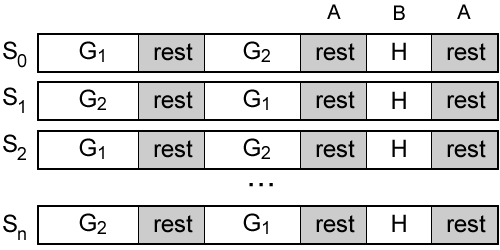
\includegraphics[width=0.6\textwidth]{figures/closing-experiment2-design.png}
%   \caption{Experimental design used in experiment 2. $S_j$ represents the $j^{\text{th}}$ subject, $G_i$ are calibration games, $COTS$ is an off-the-shelf game, and $rest$ is a resting period.}
%   \label{fig:closing-experiment2-design}
%\end{figure}

%Figure \ref{fig:closing-experiment2-design} illustrates the design of experiment 2. Each subject starts in the calibration part, where he/she plays two calibration games ($G_1$ or $G_2$) separed by a resting period (no interactions). When the subject finishes playing the calibration games, the video recordings of the subject (playing the calibration games) is processed with computer vision to extract the user signals required as input for the emotion detection model, e.g. HR and facial actions (see section \ref{sec:closing-definition-inputs}). Those extracted signals are then used to train the emotion detection model. The labeling of the signals regarding emotional states is contextualized according to the known stress and boredom aspects of the calibration games, as previously described (see sections \ref{sec:contributions} and \ref{closing:investigation-machine-learning}).

%After the model has been trained, the subject enters the emotion detection part of the experiment. In this part, the subject rests (phase A), plays a COTS game (phase B), then rests again (phase A). The video recordings of the emotion detection part is analyzed with computer vision to extract the user signals required by the emotion detection model. The extracted signals are then used as input for the previously trained emotion detection model, which outputs the estimated emotional state of the subject. The emotional state of subjects will be estimated at fixed intervals of time, e.g. every 60 seconds, throughout the emotion detection part of the experiment. Each one of those detection situations can be seen as a checkpoint. The ground truth for each checkpoint will be provided by the subjects with a self-assessment questionnaire regarding his/her current levels of stress and boredom. When a checkpoint is reached during the interaction with the COTS game, the game pauses and the questionnaire is presented to the subject. When the subject finishes answering the questionnaire, the COTS game resumes and the subject continues playing until the next checkpoint is reached.

%\begin{figure}[ht]
%    \centering
%    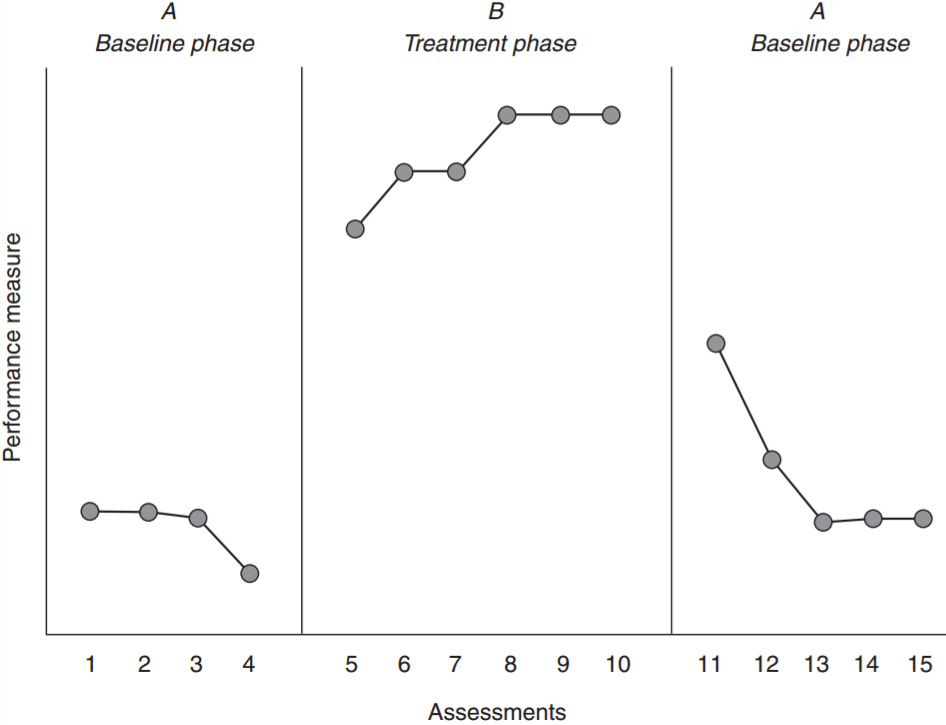
\includegraphics[width=0.85\textwidth]{figures/time-series-design-breakwell.png}
%    \caption{Time-series experimental design using an A-B-A (baseline, treatment, baseline) approach. Reproduced from \textcite{breakwell1994research}.}
%    \label{fig:time-series-design-breakwell}
%\end{figure}

%The mentioned checkpoints will be implemented using a time-series experiment design. In a time-series design there is a periodic measurement process on an individual and the introduction of a treatment into this time series of measurements results in a discontinuity in the measurements recorded in the time series \parencite{campbell2015experimental}. Figure \ref{fig:time-series-design-breakwell} illustrates the design. The A-B-A design is a common single-case time-series experimental design in which the measurements are conducted throughout the three parts of the process, i.e. A (baseline), B (treatment) and A (baseline) \parencite{robson2016real}. Phase A, referred to as the baseline phase, is a period where the subject is not under the effect of the treatment, so the measurements should reflect natural occurences. In experiment 2, it corresponds to the resting period. Phase B, referred as the treatment phase, is the period where the treatment/intervention is applied. In experiment 2, it is the interaction with the COTS game.
%In the A-B-A design, the application of a treatment followed by its removal should result in changes in the measurements among the three phases, e.g. lower values during phase A and elevated values during phase B, which confirms that the variation is a result of the treatment.

%The accuracy evaluation that confirms or refutes hypotheses \textbf{H1} and \textbf{H2} will be based on the comparison of the estimated emotional states and the self-reported emotional states informed by the subjects as ground truth during each checkpoint.

%%In the A-B-A part, the subject starts with a resting period (phase A), which is followed by the COTS treatment (phase B), finally followed by another resting period (phase A). During the A-B-A part, subjects periodically self-report their emotional state using a questionnaire, as previoslu

%%Additionally to the self-assessment of the emotional state, during the whole experiment subjects will be recorded by a video camera and monitored by a HR watch. The data collected during experiment 2 regarding the calibration games will be used to train a machine learning model, which will be used to detect the emotional state of users during the interaction with the ordinary game. The processing will be performed offline and after the experiment. Results of that analysis will prove or refute the previously mentioned hypothesis that all defined components, i.e. computer vision technique, machine learning model and calibration games, work in combination to detect emotional states.

%%During the gameplay of the non-calibration, off the shelf game the emotional state of users will be constrantly measured. Experiment 2 will produce data regarding variation of signals of subjects (from the calibration games) and ground truth data related to emotions during the gameplay of an ordinary game. The signals data will be used to train the machine learning model, which will be evaluated against the collected ground truth data (for further information regarding such validation process, see section \ref{closing:development-software}).

%%The experiment design will be based on a within-subject approach \parencite{lane2015online} where all participants perform at all levels of the treatment and there are no control groups. In the context of this research, user signals, e.g. HR, facial actions and self-reported emotional state, will be measured and used in a user-tailored model, so the division of subjects into more than one group poses a problem. Each individual will inevitably differ from one another regarding signals and emotions, such as variations in average HR during rest, for instance. Additionally people present different perceptions regarding stress and boredem. Those inherent differences pose comparision problems, so a within-subject approach simplifies the analysis of data and reduces the complexities associated with dividing subjects in different groups.

%\subsection{Challenges and unresolved issues}
%\label{experiment2-challenges}

%The first challenge regarding experiment 2 concerns the validation of the proposed method. The results of experiment 2 will demonstrate the accuracy and limitations of the proposed method, however further questioning regarding the method will innevitably surface, for instance:

%\begin{itemize}
%  \item Are all steps/signals used in the method necessary? Will a simpler and non-intrusive approach (e.g. use of remotely acquired HR information with no calibration phase) produce the same results?
%  \item Is the proposed method more accurate than an approach based on physical sensors?
%  \item Is the proposed method better than existing non-intrusive methods? It is more accurate, cheaper or easier to use?
%\end{itemize}

%Those questions could be answered with several experiments, however a direct comparison of the proposed method and existing methods is not completely plausible or viable. The proposed method relies on games as emotion elicitaion sources, which is not the case for several similar approaches that use images and sounds as stimuli. When game-like material is used as emotion elicitation sources, the context and/or the experimental design employed is different from the one proposed in experiment 2, including the use of a COTS game. Additionally a significant number of different approaches for emotion estimation exist (see chapters \ref{ch:literature-face}, \ref{ch:literature-physiological} and \ref{ch:literature-multifactorial}). Those approaches rely on different ideas, theories and signals and a direct comparison with the proposed method might not be plausible due to such differences.

%For that reason, a contextualization of the proposed method regarding existing methods is difficult. For time and resource constraints, it has been decided that an accuracy evaluation of the proposed method in comparison to a simpler emotion estimation approach based on a single signal, i.e. HR, is acceptable. It will partially answer some of the mentioned questions and provide reseachers with information to better contextualize and evaluate the feasibility of the proposed approach.

%Another challenge regarding experiment 2 is how to measure emotional states without disturbing and affecting the actual measurements. Interrupting users during gameplay is not ideal, however it is the approach described in the literature by related works. Careful planning will be required to decide the frequency and the way users will report their emotional states. If the measurements are performed too often, more data points will be available for analysis, however they might not necessarily reflect the real emotional state of users, e.g. user is bored because of the questionaire, not the game being played. If the measurements are performed too sparsely, data points will more likely reflect the real emotional state of users, however fewer data points will be available for validation.

%%Still related to emotional measurements is the decision of which questionnaire format to use in the process. As previously described, possible options are a likert scale, SAM and AS. Both SAM and AS are established and proven emotion measurement instruments, which would strengthen the theoretical foundations of the emotion measurement process. As a downside, however, they require the researcher to instruct users on how to properly answer the questionaire. User might not understand, even after the researchers explanation, what valence and arousal are, which could affect the answers and the emotion measurements. A likert scale, on the other hand, relies on the assumption that subjects know the concepts of stress and boredom within the context of games, eliminating or significantly reducing the risks of misunderstandings. If a likert scale is used, the terms ``stress" and ``boredom" can be further explained later on in the thesis using constructs of arousal and valence from established emotion theories, if that is necessary. To my understanding, a likert scale has already been successfully used in experiment 1 and is more likely to produce better results than trying to use SAM or AS as measurement tools, which risks the acquisition of answers that were misunderstood by subjects.

%Finally another unresolved issue is the COTS game to be used. Differently from the calibration games, this game should produce a natural interaction with users, causing variations of emotions that are expected from an ordinary game. The challenge is to choose a game able to elicitate sufficient variations in both boredom and stress emotional states, ortherwise the ground truth data will be skewed.

%%When measuring HR, for instance, some subjects will have higher/lower HR mean than others, independent of the group they are in or the treatment they undergo. To counter that problem, the experiment will use a one-group posttest design \cite{kirk1982experimental}, as illustrated by Figure \ref{fig:closing-experiment2-design}. Using the first row as an example, subject $S_0$ played game $G_a$ as the first level of the treatment, followed by a post-test of that game ($PT_a$), then a rest period. In the second level of the treatment, the subject played game $G_b$, followed by a post-test of that game ($PT_b$), then another rest period. Finally in the third level of the treatment, the subject played game $G_c$ followed by a post-test of that game ($PT_c$).

%%By using a one-group posttest design, each individual will perform on all levels of the treatment (play a set of different games). The within-subjects approach ensures that the differences between subjects are not interfering in the comparison, since a subject is being compared to his/herself in the different levels of the treatment. Subjects are not being compared among each other. In essence, each subject is serving as his/her own control group. According to Kirk \cite{kirk1982experimental}, the one-group posttest design should only be used when the researcher knows the mean value of the independent variable when no treatment is in effect. Such information will be obtained during the resting periods of the experiment, where the baseline value for all measured signals can be established for each subject.

%%The process of sampling a group of participants for each experiment will follow the convenience sampling approach, a non-probability sampling technique where participants are recruited because of their convenient accessibility/proximity to the researcher. Volunteers will be randomly recruited for each experiment. A probability sampling approach, where each individual of the population has an equal chance of being selected, would be ideal and would strength the external validity of the research. However the costs, logistics and time constraints associated with it makes such approach impractical in the context of this research.
